\artigotrue
\chapter{TÍTULO DO PRIMEIRO ARTIGO}
\chapternote{Este capítulo é baseado em um artigo que eu ainda não publiquei.}
\shorttitle{Primeiro artigo}
\label{chap:chapter01}

\begin{chapterabstract}{brazilian}{Palavra-chave 1. Palavra-chave 2. Palavra-chave 3}
Este é o resumo do primeiro artigo da tese. Note que as palavras-chave devem ser separadas com um \emph{ponto} 
ao invés de \emph{vírgula}.
\end{chapterabstract}

\begin{chapterabstract}{english}{Keyword 1. Keyword 2. Keyword 3}
This is the abstract of the first article of the thesis. Note that the keywords must be separated with a 
\emph{dot} instead of a \emph{comma}.
\end{chapterabstract}

\formatchapter

\section{INTRODUÇÃO}

\blindtext[2]

\subsection{Hipótese e Objetivos}

\blindtext[2]

\section{MATERIAL E MÉTODOS}

Este é um texto bem formatado, escrito em Seropédica, RJ. \blindtext[1]

Este é o código fote de uma função construída no ambiente R:

\begin{verbatim}
> soma <- function (a, b) {a + b}
> soma(2, 2)
[1] 4
\end{verbatim}

Está é uma matriz bem formatada:

\begin{equation}
  A_{m,n} =
 \begin{pmatrix}
  a_{1,1} & a_{1,2} & \cdots & a_{1,n} \\
  a_{2,1} & a_{2,2} & \cdots & a_{2,n} \\
  \vdots  & \vdots  & \ddots & \vdots  \\
  a_{m,1} & a_{m,2} & \cdots & a_{m,n}
 \end{pmatrix}
\end{equation}

\begin{subequations}\label{eq:maxwell}
E estas são as equações de Maxwell:
\begin{align}
        B'&=-\nabla \times E,\\
        E'&=\nabla \times B - 4\pi j,
\end{align}
\end{subequations}

\section{RESULTADOS}

Aqui está mais um texto bem formatado. \blindtext[1]

Que tal fazer um link para a figura \autoref{fig:ocio}? E também citar o \citeonline{Feyerabend1977} com um 
link para a localização da referência bibliográfica?

\begin{figure}[!ht]
\label{fig:ocio}
\centering
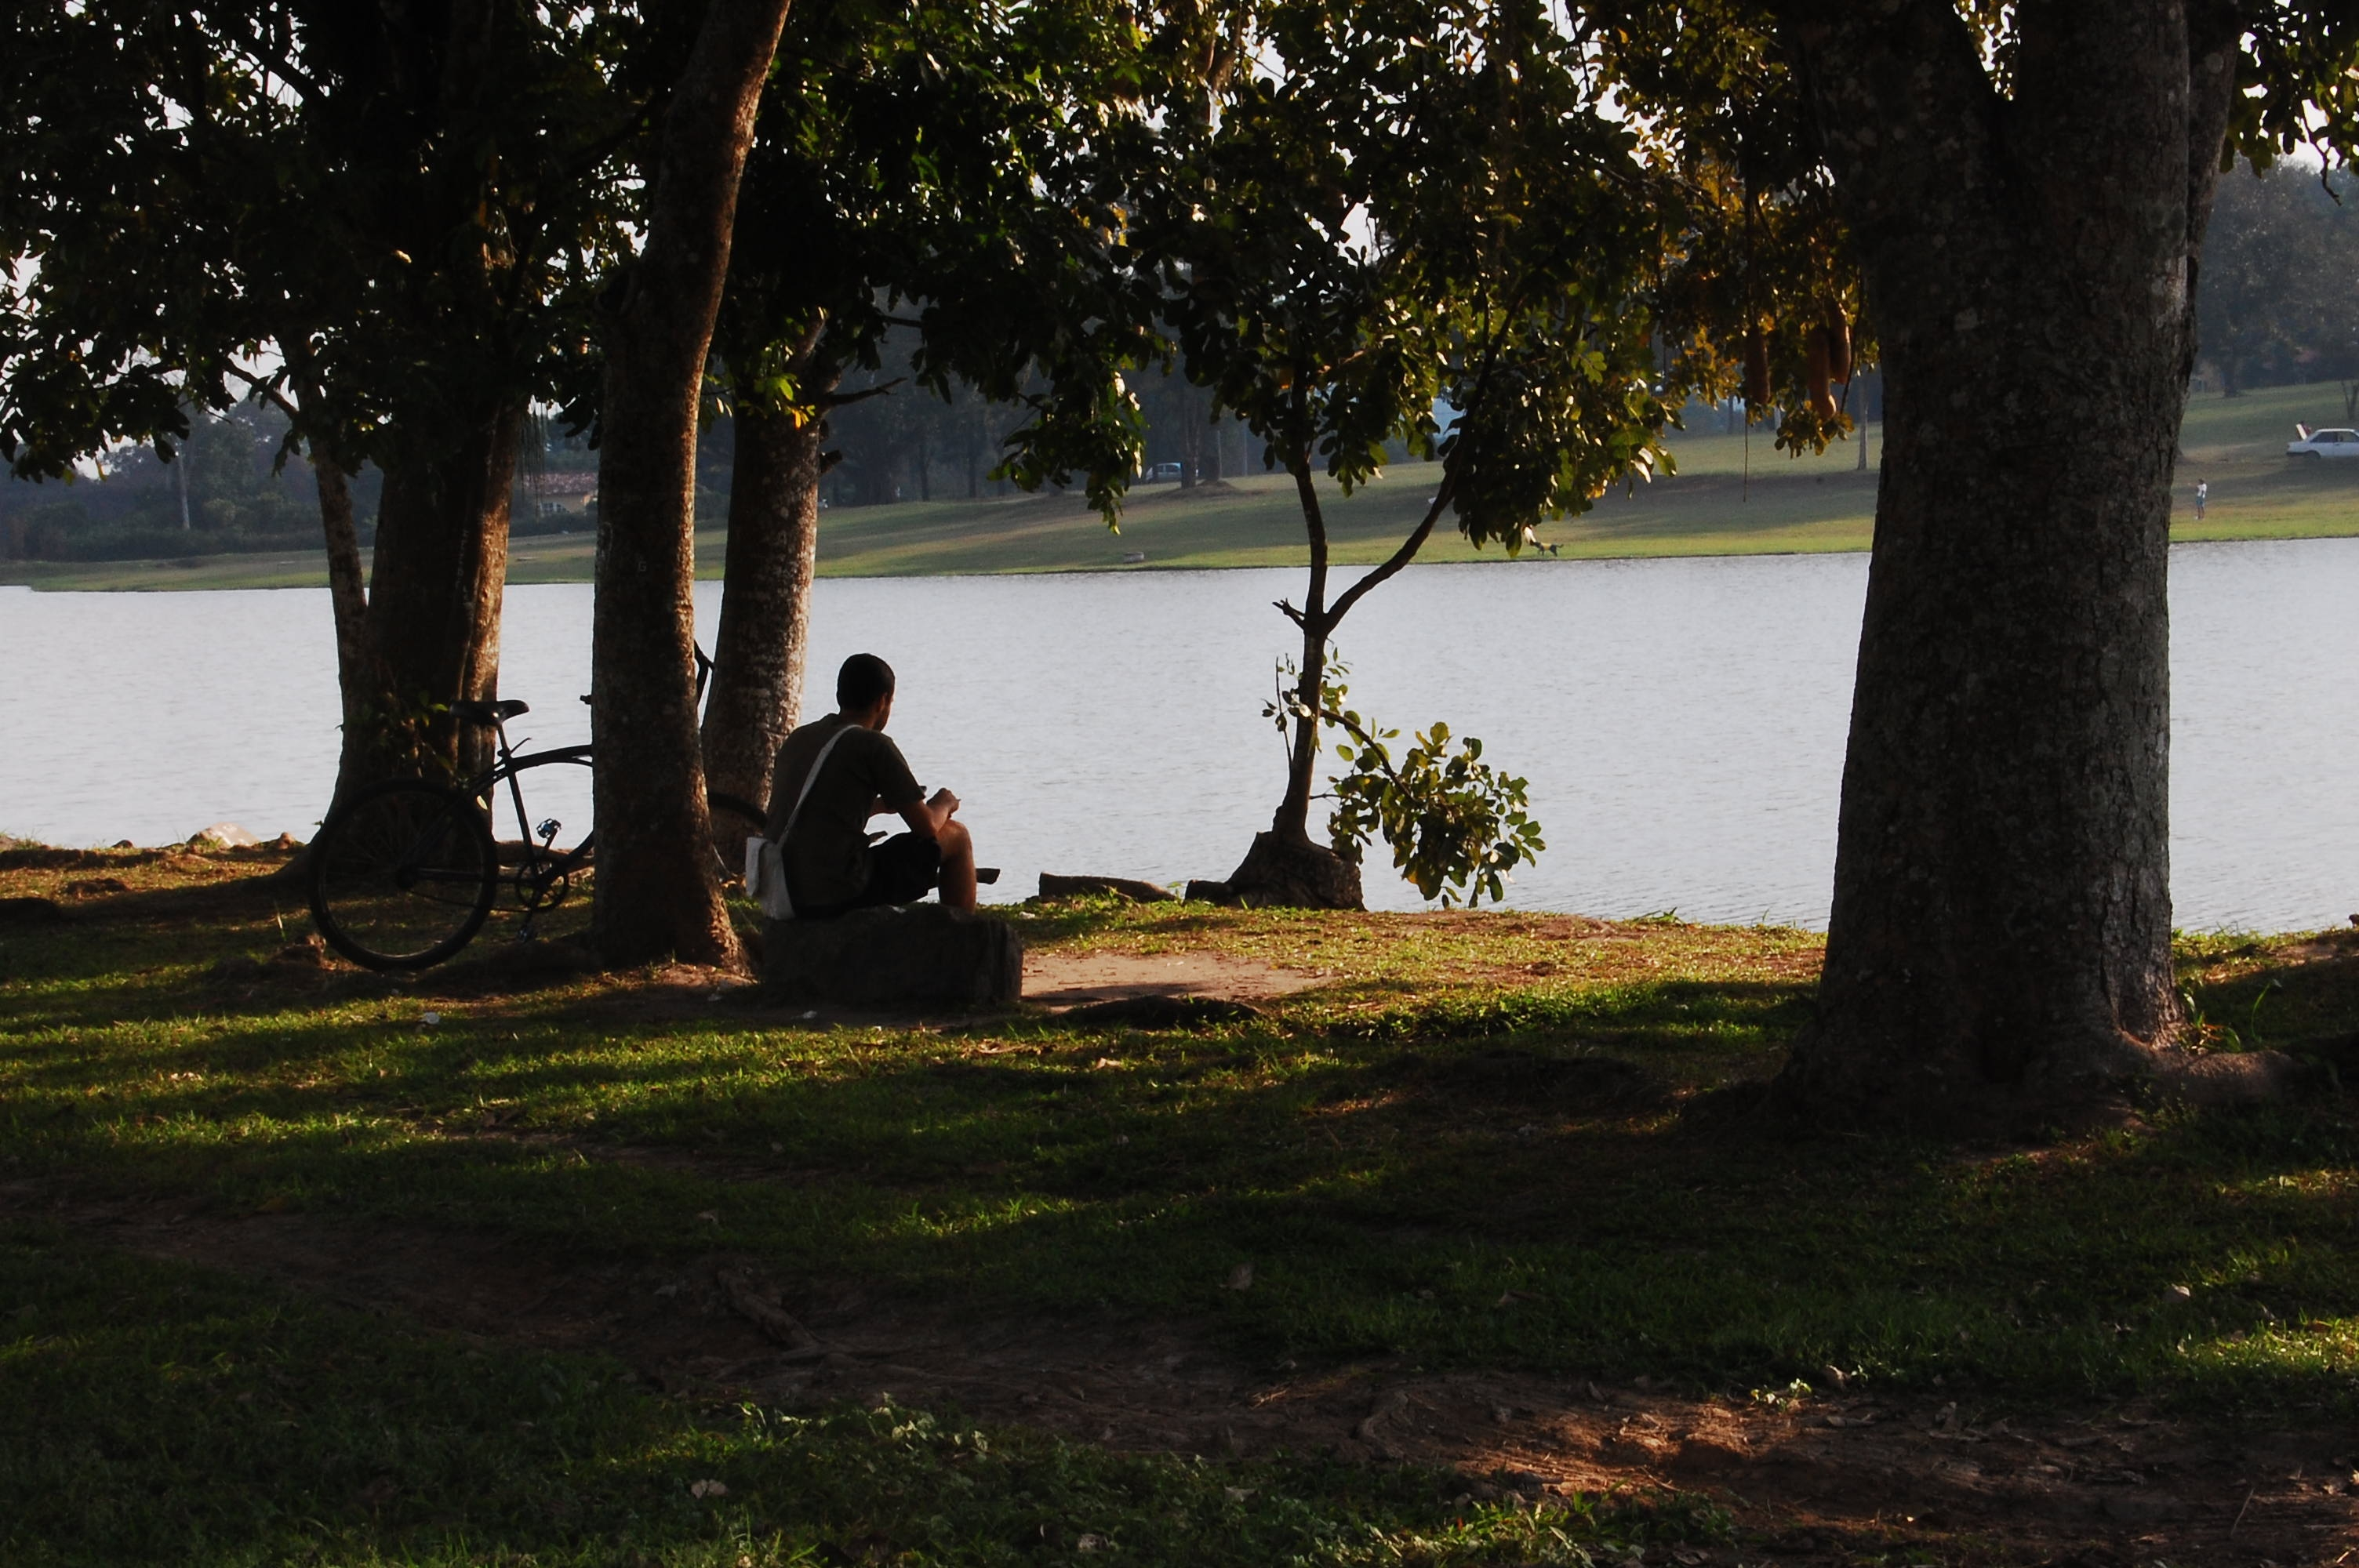
\includegraphics[width=16cm]{figura02}
\caption[O ócio criativo.]{O ócio criativo. Fonte: 
\url{http://r1.ufrrj.br/graduacao/img/acesso-2012/o-ocio-criativo.jpg}}
\end{figure}

\subsection{Outros Resultados}

\blindtext[1]

\subsubsection{Ainda outros resultados}

\blindtext[1]

\section{DISCUSSÃO}

Aqui está o último texto muito bem formatado. \blindtext[2]

Que tal fazer um link para a equação \autoref{eq:maxwell}?

\section{CONCLUSÕES}

\begin{itemize}
  \item Está é uma conclusão importante.
  \item Está é outra conclusão importante.
  \item Está é uma conclusão menos importante.
\end{itemize}
